\documentclass{article}
\usepackage[margin=1.25in]{geometry}
\usepackage{amsmath, amssymb, setspace, enumerate, enumitem}
\usepackage{setspace}
\usepackage{graphicx}
\onehalfspacing

\begin{document}
    \begin{enumerate}
        \item Exercise 1.8 in LFD
        \begin{center}
            binomial distribution tells us
        \end{center}
        \begin{align*}
            p_x &= {n \choose x} p^x q^{n-x}\\
            n &= 10\\
            x &= 0 \text{ and } x = 1\\
            p &= 0.9\\
            q &= 1 - p = 0.1\\
            p_0 &= {10 \choose 0} 0.9^0 0.1^{10} = 0.1^{10} = 1 \times 10^{-10}\\
            p_1 &= {10 \choose 1} 0.9^1 0.1^9 = 10 \times 0.9 \times 0.1^9 = 9 \times 10^{-9}\\
            p&= p_0 + p_1 = 9.1 \times 10^{-9}
        \end{align*}

        \item Exercise 1.9 in LFD\\[0.25in]
        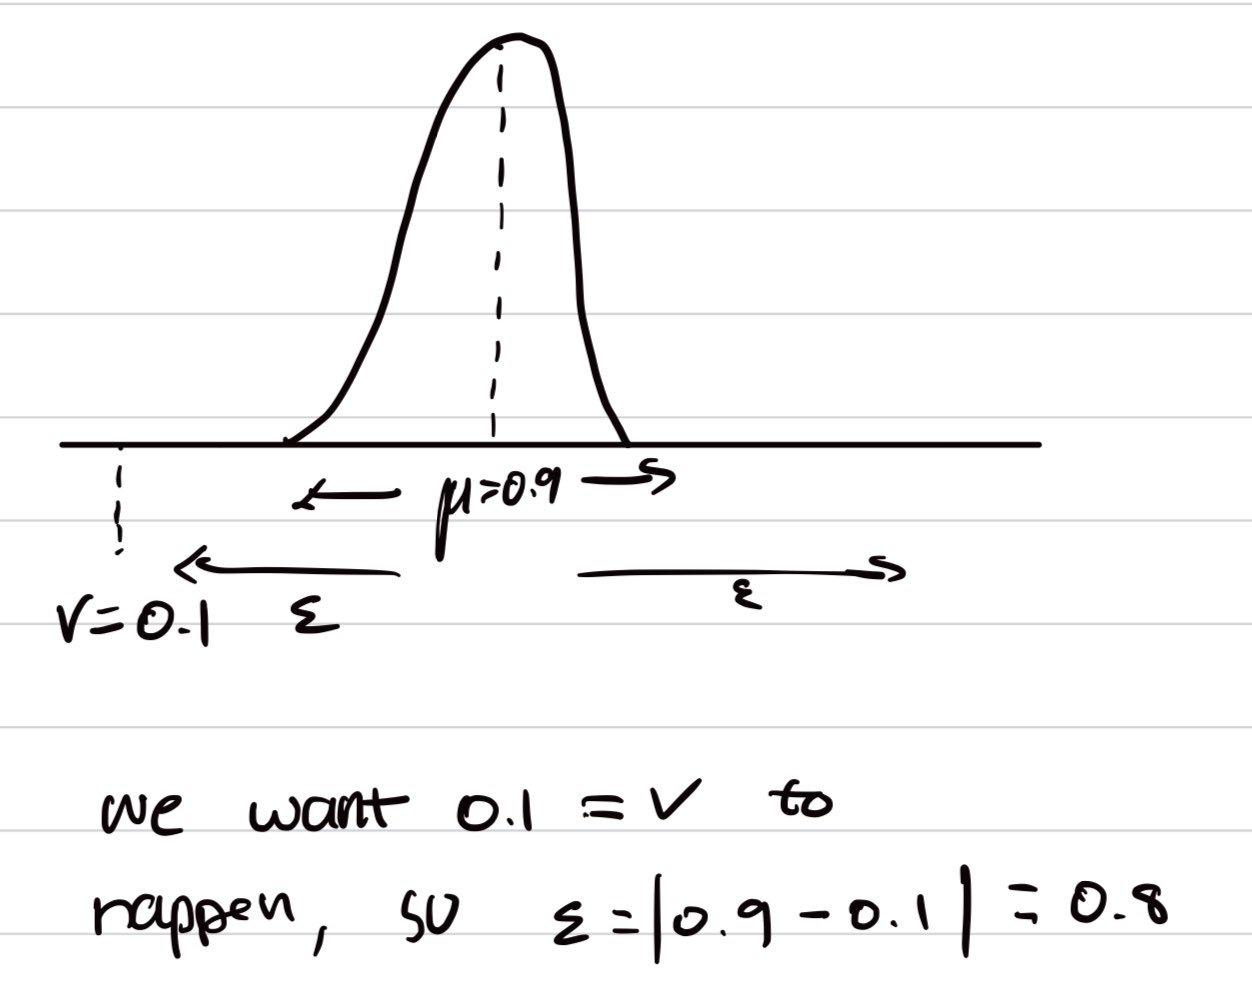
\includegraphics[scale=0.2]{images/1.9.jpg}\\[0.25in]
        Using $P[ |\nu - \mu| \geq \epsilon] \leq 2e^{-2\epsilon^2N}$, we can find the following bounds:\\
        Using $\epsilon = 0.8$ and $N = 10$, we can derive $2e^{-2\epsilon^2N} = 2e^{2(0.8)^2 \times 10}$, which equals $5.52 \times 10^{-6}$.\\
        Since this is a bound, it is reasonable for it to be greater than our answer in exercise 1.8

        \item Exercise 1.10 in LFD
        \begin{enumerate}[label=(\alph*)]
            \item $\mu = 0.5$
            \item 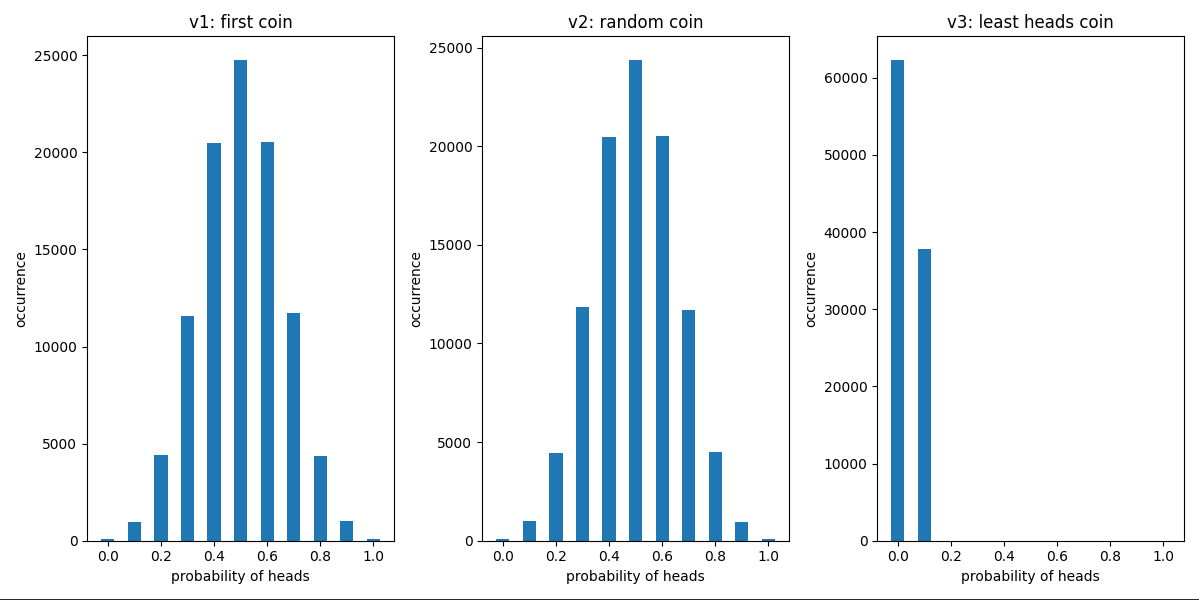
\includegraphics[scale=0.35]{images/1.10b.png}
            \item 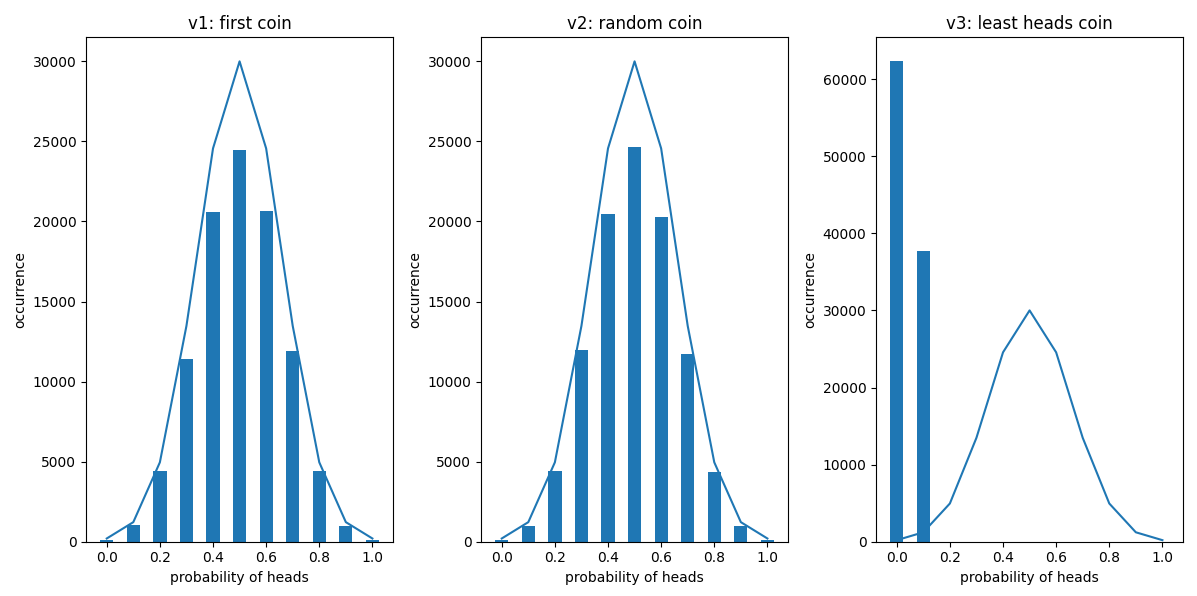
\includegraphics[scale=0.35]{images/1.10c.png}
            \item $c_1$ and $c_{rand}$ obey the Hoeffding bound, $c_{min}$ does not because $c1$ and $c_{rand}$ were selected without looking at the data, while $c_{min}$ looks at the data before selecting. $c_{min}$ represents the "unlucky" choice
            \item There are 1,000 bins with evenly distributed green and red marbles, from each bin, pick 10 marbles, we can use green marble to represent flipping heads, and red flipping tails. $c_1$ will be the first bin, $c_{rand}$ will be a random bin, and $c_{min}$ will be the bin from which you picked the most red marbles from (least green marbles / heads).
        \end{enumerate}

        \item Exercise 1.11 in LFD
        \begin{enumerate}[label=(\alph*)]
            \item No, to acheive this, we need $E_{out} \approx 0$, which means that we need $E_{in} \approx E_{out} \approx 0$. Due to the low data points, the best assumption we can make is $E_out \approx 0.5$, which tells us nothing other than random.
            \item Yes, outside the data we don't know anything about the datapoints, so if there are more points that are $-1$ outside the data than $+1$, then our hypothesis $C$ will be better than our hypothesis $S$.
            \item We need to look at all possible probabilities and pick those that have 13 or more +1 in the sample of 25. We know that $p=0.9$, so there's a 0.9 chance that a point is $+1$ and 0.1 chance a point is $-1$, so we can derive the following equation:
            \begin{center}
                $N = 25$\\
            \end{center}
            \begin{align*}
                \sum_{n=13}^N {25 \choose n} 0.9^n \times 0.1^{25-n} &\approx 0.99999\\
            \end{align*}
            \item No, the value $p$ doesn't know anything about the data outside the 25 data points, so we can't make any assumption of $C$ and $S$ outside. In the data set, $S$ will always pick the better hypothesis than $C$, so if there are more $+1$ than $-1$, it will pick $h_1$, vise-versa, so inside the data, there is no way that $C$ will product a hypothesis better than $S$.
        \end{enumerate}

        \item Exercise 1.12 in LFD
        \begin{enumerate}[label=(\alph*)]
            \item We don't know anything about the sample, so we can't make any assumptions of how well our $g$ can approximate $f$, in addition, the problem says "guarantee", which will never happen.
            \item No, in order to have a high probability that our $g$ approximates $f$ well out of sample, we need our $E_{out} \approx E_{in} \approx 0$. With $4000$, which is a small data point, we can say $E_{in} \approx 0$, but we can't say anything about $E_{out} \approx E_{in}$ since that requires $N$ to be large.
            \item \textbf{This is the best choice}, more likely than not we will declare that we have failed, we don't have enough data to say anything about outside the $N = 4000$ data points.
        \end{enumerate}

        \item Problem 1.3 in LFD
        \begin{enumerate}[label=(\alph*)]
            \item $w^*$ separates the data, so $x_n = y_n$, let $A_n = x_n = y_n$ and $p = \min_{1 \leq n \leq N} A^2_nw^*$, $A^2_n$ will always be a positive number, so $p>0$
            \item Assume
            \begin{align*}
                w^T(t)w^* &\geq w^T(t-1)w^* + p\\
                w^T(t) &= w(t-1) + y_*x_* \text{ update rule}\\
                (w^T(t-1) + y_*x_*)w^* &\geq w^T(t-1)w^* + p\\
                w^T(t-1)w^* + y_*x_*w^* &\geq w^T(t-1)w^* + p\\
            \end{align*}
                Here, we see that $w^T(t-1)w^*$ are the same on both side of the inequality, so we need to prove that $y_*x_*w^* \geq p$, but we already know that $p \leq y_n(w^{*T}x_n)$ from part (a), so the statement is true $\hfill \blacksquare$
                \\[0.25in] prove $w^T(t)w^* \geq tp$ by induction:\\
                base case: $t=0$, $w(0) = 0$, so $0\geq0$ is true\\
                induction step: assume $k=t$ and create our induction hypothesis $w^T(k)w^* \geq kp$\\
                Prove $w^T(k+1)w^* \geq (k+1)p$
                \begin{align*}
                    (w^T(k) + y_*x_*)w^* &\geq (k+1)p \text{ update rule}\\
                    w^T(k)w^* + y_*x_*w^* &\geq kp + p
                \end{align*}
                Our induction hypothesis says $w^T(k)w^* \geq kp$, and we know that $y_*x_*w^* \geq p$ from part (a), so the statement is true $\hfill \blacksquare$
            
            \item with the update rule, we get
            \begin{align*}
                ||w(t-1) + x(t-1)y(t-1)||^2 &\leq ||w(t-1)||^2 + ||x(t-1)||^2
            \end{align*}
            \begin{center}
                We can solve LHS, so
            \end{center}

            \begin{align*}
                ||[w(t-1) + x(t-1)y(t-1)]^2|| &= ||w(t-1)^2 + 2w(t-1)x(t-1)y(t-1) + x(t-1)^2y(t-1)^2||\\
                y(t-1)^2 = 1 \text{ since y } \in\{-1, 1\}\\
                &=||w(t-1)^2 + 2w(t-1)x(t-1)y(t-1) + x(t-1)^2||\\
                &||w(t-1)^2+x(t-1)^2|| \text{ is in both sides of the inequality}
            \end{align*}

            On the LHS, we have $2w(t-1)x(t-1)y(t-1)$, which, when $x(t-1)$ is misclassified by $w(t-1)$, becomes $<0$, so
            \begin{align*}
                ||w(t-1)^2 + x(t-1)^2 + \text{ negative number }|| &<||w(t-1)^2+x(t-1)^2||
            \end{align*}
            
            We know $||w(t-1)^2 + x(t-1)^2|| \leq ||w(t-1)||^2 + ||x(t-1)||^2$ by subadditivity, so $||w(t)||^2 \leq ||w(t-1)^2 + x(t-1)^2|| \leq ||w(t-1)||^2 + ||x(t-1)||^2$, by transitivity, we know \\ $||w(t)||^2 \leq ||w(t-1)||^2 + ||x(t-1)||^2 \hfill \blacksquare$
        
            \item BC $||w(0)||^2 = 0$ and $0R^2 = 0$, so $0 \leq 0$ is true\\[0.25in]
            Induction, assume induction hypothesis $||w(k)||^2 \leq kR^2$ for $k = t$, then we must prove it for $k = k + 1$\\[0.25in]
            so, $||w(k+1)||^2 \leq (k+1)R^2 = kR^2 + R^2$\\[0.25in]
            from (c), we know that $||w(k+1)||^2 \leq ||w(k)||^2 + ||x(k)||^2$, from the induction hypothesis, we know $||w(k)||^2 \leq kR^2$, so we must prove $||x(t)||^2 \leq R^2$, the problem tells us that $R$ is the max, so $R \geq x(t)$, therefore $R^2 \geq ||x(t)||^2$ as well\\[0.25in]
            so, $||w(k+1)||^2 \leq ||w(k)||^2 + ||x(k)||^2 \leq kR^2 + R^2$, by transitivity, $||w(k+1)||^2 \leq kR^2 + R^2 = (k + 1)R^2$, our induction proof is complete and we can conclude $||w(t)||^2 \leq tR^2 \hfill \blacksquare$
            
            \item modify the problem to $\frac{w^T(t)}{||w(t)||} \cdot w^* \geq \sqrt{t} \frac{p}{R} \frac{\sqrt{t}}{\sqrt{t}}$, so that it is $\frac{w^T(t)}{||w(t)||} \cdot w^* \geq \frac{pt}{R\sqrt{t}}$ \\[0.25in]
            We need to prove $A \geq C$ and $B \leq D$ for $\frac{A}{B}$ and $\frac{C}{D}$, then we can say that $\frac{A}{B} \geq \frac{C}{D}$, so from (b), we know that $w^T(t)w^* \geq pt$ and from (d), we know that $||w(t)||^2 \leq tR^2$, which simplifies to $||w(t)|| \leq \sqrt{t}R$, hence we can conlude that $\frac{w^T(t)}{||w(t)||}w^* \geq \sqrt{t} \frac{P}{R}$\\[0.25in]
            Rearranging variables to isolate $t$, we get $\frac{R^2(w^T(t)w^*)^2}{p^2||w(t)||^2} \geq t$, using the hint we are given, $w^T(t)w^* \leq ||w(t)|| ||w^*||$, $w^T(t) \cdot w^* = ||w(t)|| \cdot ||w^*|| \cdot cos \theta$, squaring both sides, we get $w^T(t)^2 \cdot w^{*2} = ||w(t)||^2 \cdot ||w^*||^2 \cdot cos^2\theta$, we know that $cos\theta$ is bounded by $\{-1, 1\}$, since it's squared, its value is always 1, therefore $w^T(t)^2 \cdot w^{*2} \leq ||w(t)||^2 \cdot ||w^*||^2$\\[0.25in]
            So, we can derive $\frac{||w(t)||^2 \cdot ||w^*||^2 R^2}{p^2 ||w(t)||^2} \geq \frac{R^2(w^T(t)w^*)^2}{p^2||w(t)||^2} \geq t$, we can simplify this to $\frac{||w^*||^2R^2}{p^2} \geq \frac{R^2(w^T(t)w^*)^2}{p^2||w(t)||^2}\geq t$, by transitivity, $\frac{R^2||w^*||^2}{p^2}\geq t \hfill \blacksquare$
        \end{enumerate}

        \item Problem 1.7 in LFD
        \begin{enumerate}[label=(\alph*)]
            \item \textbf{FINISH HERE}
            \item \textbf{FINISH HERE}
        \end{enumerate}
    \end{enumerate}
\end{document}